\documentclass{beamer}

\pdfmapfile{+sansmathaccent.map}


\mode<presentation>
{
  \usetheme{Warsaw} % or try Darmstadt, Madrid, Warsaw, Rochester, CambridgeUS, ...
  \usecolortheme{seahorse} % or try seahorse, beaver, crane, wolverine, ...
  \usefonttheme{serif}  % or try serif, structurebold, ...
  \setbeamertemplate{navigation symbols}{}
  \setbeamertemplate{caption}[numbered]
} 


%%%%%%%%%%%%%%%%%%%%%%%%%%%%
% itemize settings

\definecolor{mypink}{RGB}{255, 150, 150}
\definecolor{myblue}{RGB}{150, 150, 255}
\definecolor{mygray}{gray}{0.8}

\setbeamertemplate{itemize items}[default]

\setbeamertemplate{itemize item}{\color{mypink}$\blacksquare$}
\setbeamertemplate{itemize subitem}{\color{myblue}$\blacktriangleright$}
\setbeamertemplate{itemize subsubitem}{\color{mygray}$\blacksquare$}

%%%%%%%%%%%%%%%%%%%%%%%%%%%%
% block settings

\setbeamercolor{block title}{bg=red!30,fg=black}


%%%%%%%%%%%%%%%%%%%%%%%%%%%%
% URL settings
\hypersetup{
    colorlinks=true,
    linkcolor=blue,
    filecolor=blue,      
    urlcolor=blue,
}

%%%%%%%%%%%%%%%%%%%%%%%%%%

\renewcommand{\familydefault}{\rmdefault}

\usepackage{amsmath}
\usepackage{mathtools}

\DeclareMathOperator*{\argmin}{arg\,min}

\usepackage{subcaption}




%%%%%%%%%%%%%%%%%%%%%%%%%%%%
% code settings

\usepackage{listings}
\usepackage{color}
\definecolor{mygreen}{rgb}{0,0.6,0}
\definecolor{mygray}{rgb}{0.5,0.5,0.5}
\definecolor{mymauve}{rgb}{0.58,0,0.82}
\lstset{ 
  backgroundcolor=\color{white},   % choose the background color; you must add \usepackage{color} or \usepackage{xcolor}; should come as last argument
  basicstyle=\footnotesize,        % the size of the fonts that are used for the code
  breakatwhitespace=false,         % sets if automatic breaks should only happen at whitespace
  breaklines=true,                 % sets automatic line breaking
  captionpos=b,                    % sets the caption-position to bottom
  commentstyle=\color{mygreen},    % comment style
  deletekeywords={...},            % if you want to delete keywords from the given language
  escapeinside={\%*}{*)},          % if you want to add LaTeX within your code
  extendedchars=true,              % lets you use non-ASCII characters; for 8-bits encodings only, does not work with UTF-8
  firstnumber=0000,                % start line enumeration with line 0000
  frame=single,	                   % adds a frame around the code
  keepspaces=true,                 % keeps spaces in text, useful for keeping indentation of code (possibly needs columns=flexible)
  keywordstyle=\color{blue},       % keyword style
  language=Octave,                 % the language of the code
  morekeywords={*,...},            % if you want to add more keywords to the set
  numbers=left,                    % where to put the line-numbers; possible values are (none, left, right)
  numbersep=5pt,                   % how far the line-numbers are from the code
  numberstyle=\tiny\color{mygray}, % the style that is used for the line-numbers
  rulecolor=\color{black},         % if not set, the frame-color may be changed on line-breaks within not-black text (e.g. comments (green here))
  showspaces=false,                % show spaces everywhere adding particular underscores; it overrides 'showstringspaces'
  showstringspaces=false,          % underline spaces within strings only
  showtabs=false,                  % show tabs within strings adding particular underscores
  stepnumber=2,                    % the step between two line-numbers. If it's 1, each line will be numbered
  stringstyle=\color{mymauve},     % string literal style
  tabsize=2,	                   % sets default tabsize to 2 spaces
  title=\lstname                   % show the filename of files included with \lstinputlisting; also try caption instead of title
}

%%%%%%%%%%%%%%%%%%%%%%%%%%%%
% tikz settings

\usepackage{tikz}
\tikzset{every picture/.style={line width=0.75pt}}


\title{Unilateral constraints, friction cone}
\subtitle{Contact-aware Control, Lecture 7}
\author{by Sergei Savin}
\centering
\date{Fall 2020}



\begin{document}
\maketitle


\begin{frame}{Content}

\begin{itemize}
\item Physical contact
\item Models of physical contact
\item Friction cone
\begin{itemize}
\item Visual idea
\item Friction and normal reaction force relation
\item Algebraic approach
\end{itemize}
\item Contact point
\item Contact through a body
\begin{itemize}
\item Static case
\item Rotations
\end{itemize}
\item Violating friction cone constraint
\item Read more
\end{itemize}

\end{frame}



\begin{frame}{Physical contact}
% \framesubtitle{O}
\begin{flushleft}

\begin{figure}
    \centering
    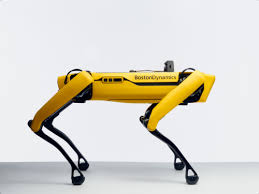
\includegraphics[width=0.45 \linewidth]{fig_SPOT.jpeg}
    \caption{Spot, a quadruped robot by Boston Dynamics}
    \label{fig:spot}
\end{figure}

Consider Spot: are its contacts well described as $\bo{g}(\bo{q}) = 0$?

\bigskip

The answer is no, as its contacts can indeed break from the constraint manifold $\bo{g}(\bo{q}) = 0$. In particular, its feet can move up. They can't move down, however. And if they want to move sideways, they will have to first produce enough force to overcome static friction.

\end{flushleft}
\end{frame}


\begin{frame}{Models of physical contact}
% \framesubtitle{O}
\begin{flushleft}

Typical contact models that come close to describing real world physical contact are:

\begin{figure}
    \centering
    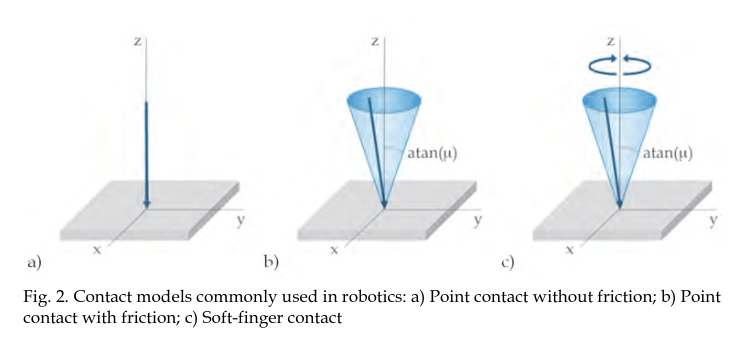
\includegraphics[width= \linewidth]{fig2.png}
    % \caption{}
    \label{fig:contact}
\end{figure}

\scriptsize{Picture is from \emph{Sancho-Bru, J.L., P\'{e}rez-Gonz\'{a}lez, A., Mora, M.C., L\'{o}n, B.E., Vergara, M., Iserte, J.L., Rodriguez-Cervantes, P.J. and Morales, A., 2011. Towards a realistic and self-contained biomechanical model of the hand. In Theoretical biomechanics. IntechOpen.}}

\end{flushleft}
\end{frame}



\begin{frame}{Friction cone}
\framesubtitle{Visual idea}
\begin{flushleft}

You can visualize friction cone as all possible reaction forces, acting at the contact point:

\begin{figure}
    \centering
    

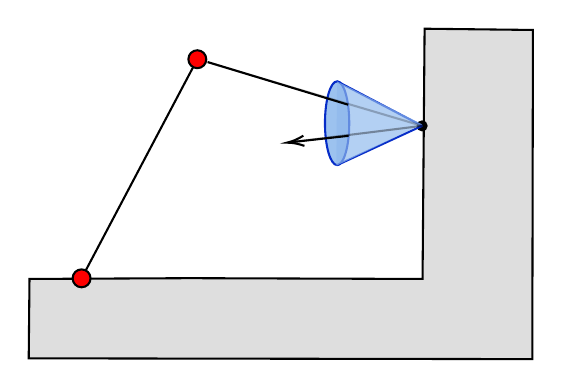
\begin{tikzpicture}[x=0.75pt,y=0.75pt,yscale=-0.75,xscale=0.75]
%uncomment if require: \path (0,300); %set diagram left start at 0, and has height of 300

%Straight Lines [id:da511009501867824] 
\draw    (150.25,190.35) -- (224.6,49.6) ;
%Shape: Polygon [id:ds12621320375323086] 
\draw  [fill={rgb, 255:red, 222; green, 222; blue, 222 }  ,fill opacity=1 ] (440.2,30.8) -- (370.6,30) -- (369.29,190.75) -- (219.79,190.25) -- (116.79,190.75) -- (116.29,241.75) -- (439.79,242.25) -- cycle ;
%Shape: Circle [id:dp8262097043760679] 
\draw  [fill={rgb, 255:red, 0; green, 0; blue, 0 }  ,fill opacity=1 ] (366.13,92.4) .. controls (366.13,90.81) and (367.41,89.53) .. (369,89.53) .. controls (370.59,89.53) and (371.88,90.81) .. (371.88,92.4) .. controls (371.88,93.99) and (370.59,95.28) .. (369,95.28) .. controls (367.41,95.28) and (366.13,93.99) .. (366.13,92.4) -- cycle ;
%Shape: Circle [id:dp2680036705913309] 
\draw  [fill={rgb, 255:red, 255; green, 0; blue, 0 }  ,fill opacity=1 ] (144.5,190.35) .. controls (144.5,187.17) and (147.07,184.6) .. (150.25,184.6) .. controls (153.43,184.6) and (156,187.17) .. (156,190.35) .. controls (156,193.53) and (153.43,196.1) .. (150.25,196.1) .. controls (147.07,196.1) and (144.5,193.53) .. (144.5,190.35) -- cycle ;
%Shape: Ellipse [id:dp3954723668349849] 
\draw  [color={rgb, 255:red, 0; green, 39; blue, 198 }  ,draw opacity=0.97 ][fill={rgb, 255:red, 156; green, 194; blue, 239 }  ,fill opacity=1 ] (306.6,90.7) .. controls (306.6,75.84) and (310.09,63.8) .. (314.4,63.8) .. controls (318.71,63.8) and (322.2,75.84) .. (322.2,90.7) .. controls (322.2,105.56) and (318.71,117.6) .. (314.4,117.6) .. controls (310.09,117.6) and (306.6,105.56) .. (306.6,90.7) -- cycle ;
%Straight Lines [id:da41806140316108764] 
\draw [color={rgb, 255:red, 0; green, 39; blue, 198 }  ,draw opacity=0.97 ][fill={rgb, 255:red, 156; green, 194; blue, 239 }  ,fill opacity=1 ]   (314.4,63.8) -- (369,92.4) ;
%Straight Lines [id:da8734911464392034] 
\draw [color={rgb, 255:red, 0; green, 39; blue, 198 }  ,draw opacity=0.97 ][fill={rgb, 255:red, 156; green, 194; blue, 239 }  ,fill opacity=1 ]   (314.4,117.6) -- (369,92.4) ;

%Flowchart: Merge [id:dp07751328773533905] 
\draw  [color={rgb, 255:red, 0; green, 0; blue, 0 }  ,draw opacity=0 ][fill={rgb, 255:red, 143; green, 185; blue, 237 }  ,fill opacity=0.68 ] (314.4,63.8) -- (313.88,118.01) -- (369.01,91.43) -- cycle ;
%Straight Lines [id:da8106680503102979] 
\draw [color={rgb, 255:red, 0; green, 0; blue, 0 }  ,draw opacity=0.24 ]   (224.6,49.6) -- (369,92.4) ;
%Straight Lines [id:da5735853405821096] 
\draw [color={rgb, 255:red, 0; green, 0; blue, 0 }  ,draw opacity=0.36 ]   (369,92.4) -- (282.2,103.2) ;
%Straight Lines [id:da788051954899972] 
\draw    (321.8,98.8) -- (284.19,102.98) ;
\draw [shift={(282.2,103.2)}, rotate = 353.65999999999997] [color={rgb, 255:red, 0; green, 0; blue, 0 }  ][line width=0.75]    (10.93,-3.29) .. controls (6.95,-1.4) and (3.31,-0.3) .. (0,0) .. controls (3.31,0.3) and (6.95,1.4) .. (10.93,3.29)   ;
%Straight Lines [id:da2615117595464225] 
\draw    (231.29,51.43) -- (321.4,78.8) ;
%Shape: Circle [id:dp33456176340238253] 
\draw  [fill={rgb, 255:red, 255; green, 0; blue, 0 }  ,fill opacity=1 ] (218.85,49.6) .. controls (218.85,46.42) and (221.42,43.85) .. (224.6,43.85) .. controls (227.78,43.85) and (230.35,46.42) .. (230.35,49.6) .. controls (230.35,52.78) and (227.78,55.35) .. (224.6,55.35) .. controls (221.42,55.35) and (218.85,52.78) .. (218.85,49.6) -- cycle ;




\end{tikzpicture}

    % \caption{}
    \label{fig:contact}
\end{figure}

You can think of it as a cone, pointing at the contact surface at the right angle (perpendicular), whole angle is proportional to the friction coefficient.

\end{flushleft}
\end{frame}





\begin{frame}{Friction cone}
\framesubtitle{Friction and normal reaction force relation}
\begin{flushleft}

\begin{figure}
    \centering
    

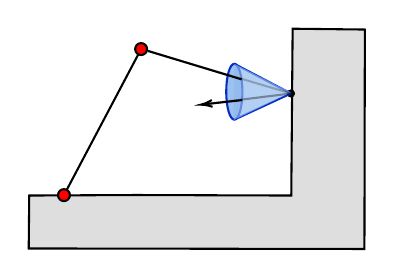
\begin{tikzpicture}[x=0.75pt,y=0.75pt,yscale=-0.5,xscale=0.5]
%uncomment if require: \path (0,300); %set diagram left start at 0, and has height of 300

%Straight Lines [id:da511009501867824] 
\draw    (150.25,190.35) -- (224.6,49.6) ;
%Shape: Polygon [id:ds12621320375323086] 
\draw  [fill={rgb, 255:red, 222; green, 222; blue, 222 }  ,fill opacity=1 ] (440.2,30.8) -- (370.6,30) -- (369.29,190.75) -- (219.79,190.25) -- (116.79,190.75) -- (116.29,241.75) -- (439.79,242.25) -- cycle ;
%Shape: Circle [id:dp8262097043760679] 
\draw  [fill={rgb, 255:red, 0; green, 0; blue, 0 }  ,fill opacity=1 ] (366.13,92.4) .. controls (366.13,90.81) and (367.41,89.53) .. (369,89.53) .. controls (370.59,89.53) and (371.88,90.81) .. (371.88,92.4) .. controls (371.88,93.99) and (370.59,95.28) .. (369,95.28) .. controls (367.41,95.28) and (366.13,93.99) .. (366.13,92.4) -- cycle ;
%Shape: Circle [id:dp2680036705913309] 
\draw  [fill={rgb, 255:red, 255; green, 0; blue, 0 }  ,fill opacity=1 ] (144.5,190.35) .. controls (144.5,187.17) and (147.07,184.6) .. (150.25,184.6) .. controls (153.43,184.6) and (156,187.17) .. (156,190.35) .. controls (156,193.53) and (153.43,196.1) .. (150.25,196.1) .. controls (147.07,196.1) and (144.5,193.53) .. (144.5,190.35) -- cycle ;
%Shape: Ellipse [id:dp3954723668349849] 
\draw  [color={rgb, 255:red, 0; green, 39; blue, 198 }  ,draw opacity=0.97 ][fill={rgb, 255:red, 156; green, 194; blue, 239 }  ,fill opacity=1 ] (306.6,90.7) .. controls (306.6,75.84) and (310.09,63.8) .. (314.4,63.8) .. controls (318.71,63.8) and (322.2,75.84) .. (322.2,90.7) .. controls (322.2,105.56) and (318.71,117.6) .. (314.4,117.6) .. controls (310.09,117.6) and (306.6,105.56) .. (306.6,90.7) -- cycle ;
%Straight Lines [id:da41806140316108764] 
\draw [color={rgb, 255:red, 0; green, 39; blue, 198 }  ,draw opacity=0.97 ][fill={rgb, 255:red, 156; green, 194; blue, 239 }  ,fill opacity=1 ]   (314.4,63.8) -- (369,92.4) ;
%Straight Lines [id:da8734911464392034] 
\draw [color={rgb, 255:red, 0; green, 39; blue, 198 }  ,draw opacity=0.97 ][fill={rgb, 255:red, 156; green, 194; blue, 239 }  ,fill opacity=1 ]   (314.4,117.6) -- (369,92.4) ;

%Flowchart: Merge [id:dp07751328773533905] 
\draw  [color={rgb, 255:red, 0; green, 0; blue, 0 }  ,draw opacity=0 ][fill={rgb, 255:red, 143; green, 185; blue, 237 }  ,fill opacity=0.68 ] (314.4,63.8) -- (313.88,118.01) -- (369.01,91.43) -- cycle ;
%Straight Lines [id:da8106680503102979] 
\draw [color={rgb, 255:red, 0; green, 0; blue, 0 }  ,draw opacity=0.24 ]   (224.6,49.6) -- (369,92.4) ;
%Straight Lines [id:da5735853405821096] 
\draw [color={rgb, 255:red, 0; green, 0; blue, 0 }  ,draw opacity=0.36 ]   (369,92.4) -- (282.2,103.2) ;
%Straight Lines [id:da788051954899972] 
\draw    (321.8,98.8) -- (284.19,102.98) ;
\draw [shift={(282.2,103.2)}, rotate = 353.65999999999997] [color={rgb, 255:red, 0; green, 0; blue, 0 }  ][line width=0.75]    (10.93,-3.29) .. controls (6.95,-1.4) and (3.31,-0.3) .. (0,0) .. controls (3.31,0.3) and (6.95,1.4) .. (10.93,3.29)   ;
%Straight Lines [id:da2615117595464225] 
\draw    (231.29,51.43) -- (321.4,78.8) ;
%Shape: Circle [id:dp33456176340238253] 
\draw  [fill={rgb, 255:red, 255; green, 0; blue, 0 }  ,fill opacity=1 ] (218.85,49.6) .. controls (218.85,46.42) and (221.42,43.85) .. (224.6,43.85) .. controls (227.78,43.85) and (230.35,46.42) .. (230.35,49.6) .. controls (230.35,52.78) and (227.78,55.35) .. (224.6,55.35) .. controls (221.42,55.35) and (218.85,52.78) .. (218.85,49.6) -- cycle ;




\end{tikzpicture}

    % \caption{}
    \label{fig:contact}
\end{figure}

Let $\bo{f}_n$ be the normal component (perpendicular to the surface locally) of the reaction force, also known as normal reaction; and let $\bo{f}_{fr}$ be tangential component (a vector lying in the tangent plane to the surface, constructed at the contact point), or friction force.

\bigskip

Then we can define a friction model as follows:

\begin{equation}
    ||\bo{f}_{fr}|| \leq \mu ||\bo{f}_n||
\end{equation}

\end{flushleft}
\end{frame}




\begin{frame}{Friction cone}
\framesubtitle{Algebraic approach, part 1}
\begin{flushleft}

Note that expression $||\bo{f}_{fr}|| \leq \mu ||\bo{f}_n||$ \emph{does not} describe friction cone, nor represents a realistic contact. The reason is: it doesn't limit the direction of the normal reaction force.

\bigskip

One way to remedy it is to first define normal direction that points from the surface as a unit vector $\bo{n}$, and then add two unit vectors that represent a basis in the tangent plane to the surface: $\tau_1$, $\tau_2$. Note that $\tau_1$ and $\tau_2$ can be found as a null space of $\bo{n}$, considering the latter as a matrix with a single column vector.

\bigskip

Then we define total reaction force as $\bo{f}$, $\bo{f}_n = \bo{n}(\bo{n}^\top \bo{f})$ and $\bo{f}_{fr} = \bo{T}(\bo{T}^\top \bo{f})$ where $\bo{T} = [\tau_1 \ \tau_2]$.

\end{flushleft}
\end{frame}




\begin{frame}{Friction cone}
\framesubtitle{Algebraic approach, part 2}
\begin{flushleft}

With that, we can define friction cone as follows:

\begin{equation}
\label{eq:friction_cone}
    || [\tau_1 \ \tau_2]^\top \bo{f} || \leq \mu \bo{n}^\top \bo{f}
\end{equation}

Note that $\bo{n}^\top \bo{f}$ is a scalar and represents norm of the normal reaction force as long as normal reaction and the normal unit vector $\bo{n}$ have a positive dot product. But if they don't, it means that the friction cone is violated, so this scenario is of no interest to us. In fact, \eqref{eq:friction_cone} prevents this, since if the mentioned above dot product is negative, the condition will never hold, as its left-hand-side is always positive, being a norm.

\end{flushleft}
\end{frame}





\begin{frame}{Friction cone}
\framesubtitle{Algebraic approach, part 3}
\begin{flushleft}

Notice that this expression:

\begin{equation}
\label{eq:friction_cone_2}
    || [\tau_1 \ \tau_2]^\top \bo{f} || \leq \mu \bo{n}^\top \bo{f}
\end{equation}

...assumes that your \emph{decision variable} is $\bo{f}$. This is a good parameterization choice, but not the only one. Another one is the following:

\begin{equation}
\label{eq:friction_cone_3}
\begin{cases}
    \sqrt{t_1^2 + t_2^2} \leq \mu n \\
    \bo{f}_{fr} = t_1 \tau_1 + t_2 \tau_2 \\
    \bo{f}_n = n \bo{n}  
\end{cases}
\end{equation}

Unlike the previous one, this representation is explicit with respect to the basis in which the forces are expressed (namely, basis is formed by vectors $\tau_1$, $\tau_2$, $\bo{n} $). This gives us an advantage in making expressions for the conic constraint simpler.

\end{flushleft}
\end{frame}



\begin{frame}{Contact point}
% \framesubtitle{Algebraic approach, part 3}
\begin{flushleft}

Assume you have a single point $K$ at which the contact takes place. This contact takes away 3 DoF of the robot:

\begin{equation}
    \begin{cases}
    x_K(\bo{q}) = x_K(0) \\
    y_K(\bo{q}) = y_K(0) \\
    z_K(\bo{q}) = z_K(0)
    \end{cases}
\end{equation}

Now assume that there is no friction, and the contact only prevents motion in the normal direction $\bo{n}$ to the contact surface. Then the contact only takes away one DoF:

\begin{equation}
    \bo{n}^\top \bo{r}_K(\bo{q}) = g_K(\bo{q})
\end{equation}

\end{flushleft}
\end{frame}




\begin{frame}{Contact through a body}
\framesubtitle{Static case}
\begin{flushleft}

You can describe contact point as restricting motion of a single point, as was suggested on the previous slide. Alternatively, you can describe a contact integration in terms of the restriction it places on the body coming in contact. 

\bigskip

For example, here is a 6-DoF contact, which prevents all motion (this is a constraint for robot's feet when they rest on the ground, or the end effector when it rests on the immobile surface it holds onto):

\begin{equation}
    \begin{cases}
    x_K(\bo{q}) = x_K(0), \ \  y_K(\bo{q}) = y_K(0),  \ \ z_K(\bo{q}) = z_K(0) \\
    \varphi_K(\bo{q}) = \varphi_K(0), \ \ \theta_K(\bo{q})  = \theta_K(0), \ \ \psi_K(\bo{q})    = \psi_K(0)
    \end{cases}
\end{equation}

where $\varphi_K$, $\theta_K$, $\psi_K$ are Euler angles of the body in contact. 

\end{flushleft}
\end{frame}



\begin{frame}{Contact through a body}
\framesubtitle{Static case, part 1}
\begin{flushleft}

Assume the body has points $K_1$, $K_2$, ..., $K_k$, where $k \geq 3$ and the points are not lying on the same line. Then it is possible to define a constraint that makes the body static by requiring all those points to be static:

\begin{equation}
    \begin{cases}
    x_{K, i}(\bo{q}) = x_{K, i}(0) \\
    y_{K, i}(\bo{q}) = y_{K, i}(0) \\
    z_{K, i}(\bo{q}) = z_{K, i}(0), \ i = 1, \ ... \ k
    \end{cases}
\end{equation}

\end{flushleft}
\end{frame}



\begin{frame}{Contact through a body}
\framesubtitle{Static case, part 2}
\begin{flushleft}

Note that increasing the number of non-colinear points beyond three doesn't change the fact that the body is stable. But there are two important observations here:

\begin{itemize}
    \item Number of points will make a difference if there are a friction cone constraints on the reaction force.
    \item Different choice of contact points will lead to different constraints expressions, and hence different Jacobians and different Cartesian reaction forces.
\end{itemize}

\end{flushleft}
\end{frame}





\begin{frame}{Contact through a body}
\framesubtitle{Rotations}
\begin{flushleft}

Consider a 4-DoF contact, which prevents motion of the contact point and the rotation of the body around the axis parallel to the: 


\begin{equation}
    \begin{cases}
    \bo{n}^\top \omega_K = 0 \\  
    x_K(\bo{q}) = x_K(0) \\
    y_K(\bo{q}) = y_K(0) \\
    z_K(\bo{q}) = z_K(0)
    \end{cases}
\end{equation}

where $\omega_K$ is the angular velocity of the body. You can prove it that it is impossible to write that constraint in terms of the orientations, since there is no function of the orientation that is being preserved under this constraint. 

\end{flushleft}
\end{frame}



\begin{frame}{Contact through a body}
\framesubtitle{Rotations, remarks}
\begin{flushleft}

\begin{equation}
    \bo{n}^\top \omega_K = 0
\end{equation}

It is a \emph{kinematic constraint}, and to appreciate the difference we can remember that previously we differentiated out constraints twice to achieve the desired DAE form; here we would only need to differentiate once.

\bigskip

Hence, our mathematics would need to be checked or re-worked, before we can use these constraints.

\end{flushleft}
\end{frame}



\begin{frame}{Violating friction cone constraint}
% \framesubtitle{Algebraic approach, part 3}
\begin{flushleft}

As implied by their name, unilateral constraints don't always hold. Here are basic scenarios when they are violated:

\begin{itemize}
    \item The force required to maintain the constraint is such that $\bo{n}^\top \bo{f}$ would have been negative. This means that the contact is lost (disengaged).
    \item The force required to maintain the constraint lies outside of the friction cone, while $\bo{n}^\top \bo{f}$ is still positive. This means that the contact point slides along the contact surface. This can be modelled as contact with no static friction discussed previously, but with  additional sliding friction force (often modelled as being proportional to the normal reaction force, sometimes dependant on the velocity of the sliding motion.
\end{itemize}

\end{flushleft}
\end{frame}



\begin{frame}{Read more}
% \framesubtitle{Parameter estimation}
\begin{flushleft}

You can read more at:

\begin{itemize}
    \item \href{https://scaron.info/teaching/friction-cones.html}{Friction cones - Stephane Caron}
\end{itemize}

\end{flushleft}
\end{frame}




\begin{frame}
\centerline{Lecture slides are available via Moodle.}
\bigskip
\centerline{You can help improve these slides at:}
\centerline{\href{https://github.com/SergeiSa/Contact-Aware-Control-Slides-Fall-2020}{github.com/SergeiSa/Contact-Aware-Control-Slides-Fall-2020}}
\bigskip
\centerline{Check Moodle for additional links, videos, textbook suggestions.}
\end{frame}

\end{document}
